\documentclass[conference]{IEEEtran}
\usepackage[utf8]{inputenc}
\usepackage[T1]{fontenc}
\usepackage[spanish,es-nodecimaldot,es-noshorthands,es-tabla]{babel}
\usepackage{amsmath,amssymb}
\usepackage{graphicx}
\usepackage{booktabs}
\usepackage{pgfplots}
\pgfplotsset{compat=1.18}
\usepackage[hidelinks]{hyperref}
\usepackage{url}
\usepackage{newunicodechar}
\newunicodechar{°}{\ensuremath{^\circ}}
\renewcommand\IEEEkeywordsname{Palabras clave}

\begin{document}

\title{Capa de atmósfera para un simulador de la ruta de \emph{Perseverance} en el cráter Jezero: modelo físico, visualización y cálculo de rutas}

\author{\IEEEauthorblockN{\textit{Nombre completo del autor}}
\IEEEauthorblockA{\textit{Escuela / carrera, universidad}\\
\textit{correo institucional}}}

\maketitle

\begin{abstract}
Se describe la capa \emph{Atmósfera} de un simulador de realidad virtual de la ruta de \emph{Perseverance} en el cráter Jezero, Marte. La capa calcula, en cada punto del terreno real (modelo de elevación HiRISE), cinco parámetros: fracción de oxígeno, dosis de radiación, temperatura del aire, presión y opacidad del polvo. Los valores base provienen de mediciones publicadas de los instrumentos MEDA, RAD y SAM; la variación de un lugar a otro se modela con leyes físicas (fórmula barométrica, ley de Beer--Lambert, ley del coseno de Lambert) y, donde no hay datos, con campos sintéticos que se identifican como tales. Se presentan los cálculos paso a paso en el punto de partida de la ruta del equipo (sol~1063), el cálculo de pendientes por diferencias centrales y su respuesta en frecuencia, la integración numérica usada para la neblina, y la comparación de tres caminos entre los sols 1063 y 1116 con una función de costo y el algoritmo A*. La recta entre los extremos es 33\,\% más corta que la ruta real pero cruza una pendiente de 18°; el camino óptimo respeta el límite de 15° y reduce el costo en 31\,\% respecto a la ruta real. Por último, se escriben en variables de estado los filtros implementados y se propone un lazo de control térmico para el traje.
\end{abstract}

\begin{IEEEkeywords}
Marte, Jezero, MEDA, modelo atmosférico, diferencias finitas, A*, variables de estado, realidad virtual.
\end{IEEEkeywords}

\section{Introducción}
El simulador \emph{Mars Route Walker} reconstruye la ruta de \emph{Perseverance} sobre el modelo de elevación HiRISE de 1\,m y permite recorrerla en realidad virtual. Sobre ese núcleo, cada integrante del equipo agrega una \emph{capa}. La capa Atmósfera responde a la pregunta \emph{¿cómo es el aire donde estoy parado?} con un panel de cinco valores y cinco vistas de falso color (calor, radiación, oxígeno, presión y polvo), implementadas en Godot~4.7~\cite{godot}.

El equipo trabaja sobre el tramo \textbf{A = sol 1063} a \textbf{B = sol 1116}. Mientras el jugador está en ese tramo, el mapa de valores de la capa (una grilla de $160\times160$ casillas de 20\,m, 3.2\,km de lado) queda fijo y centrado en él.

\textbf{Alcance y honestidad del modelo.} Los valores base y su ciclo estacional se toman de publicaciones de los equipos de los instrumentos. En la realidad, la radiación, el oxígeno y el polvo de fondo casi no cambian en pocos kilómetros; por eso la variación espacial de esos parámetros es \emph{sintética} (ruido suave de amplitud acotada) y sirve para ilustrar. La excepción es la presión, cuya dependencia con la altura es física. La Tabla~\ref{tab:fuentes} resume qué es medido y qué es sintético.

\begin{table}[t]
\caption{Valores base, fuentes y naturaleza de la variación espacial}
\label{tab:fuentes}
\centering\small
\begin{tabular}{@{}p{1.25cm}p{3.05cm}p{3.0cm}@{}}
\toprule
Parámetro & Base (fuente) & Variación espacial \\ \midrule
Presión & Ciclo estacional MEDA~\cite{harri2024} & Física: $e^{-h/H}$ \\
O$_2$ & 0.16\,\% del aire, SAM~\cite{trainer2019} & Sintética $\pm12$\,\% \\
Radiación & 0.67\,mSv/día, RAD~\cite{hassler2014} & Presión~\cite{guo2017} + sintética $\pm10$\,\% \\
Temperatura & Ciclo diario MEDA~\cite{munguira2023} & Ladera al sol / hondonada (base física) \\
Polvo $\tau$ & MEDA/TIRS~\cite{smith2023}, tormentas~\cite{sanchezlavega2025} & Parches sintéticos ($\le0.15$) + remolinos~\cite{hueso2023,toledo2023,jackson2021} \\
\bottomrule
\end{tabular}
\end{table}

\section{Tiempo: sol, estación y hora local}
\subsection{Del sol a la longitud solar $L_s$}
La estación se expresa con la longitud solar $L_s$. El modelo interpola linealmente entre anclas publicadas~\cite{harri2024,sanchezlavega2025} dentro de un año marciano de 668.6 sols:
\begin{equation}
L_s(s) = L_{s,i} + \frac{s' - s_i}{s_{i+1}-s_i}\,(L_{s,i+1}-L_{s,i}),\quad s' = s \bmod 668.6 .
\end{equation}
Para el sol 1063: $s' = 1063 - 668.6 = 394.4$, entre las anclas $(313, 153°)$ y $(565, 308°)$:
$L_s = 153 + (394.4-313)\cdot 155/252 = \mathbf{203.07°}$ (otoño del hemisferio norte).

\subsection{Hora local a partir del sol de la escena}
El núcleo ilumina la escena con un sol fijo a $35°$ de elevación, hacia el este. En el equinoccio, $\sin e = \cos\varphi\cos H$, con $\varphi$ la latitud y $H$ el ángulo horario. Con $\varphi = 18.4°$:
$\cos H = \sin 35°/\cos 18.4° = 0.5736/0.9489 = 0.6045 \Rightarrow H = 52.8° = 3.52$\,h,
y como el sol está al este, la hora local es $12 - 3.52 = \mathbf{08{:}29}$.

\section{Modelo físico y cálculos en el punto A}
Todos los números de esta sección se obtuvieron con la herramienta de análisis de la capa (\texttt{informe/analisis\_ruta.gd}), que usa las mismas funciones que el panel. En A: $x=-6965.9$\,m, $z=-2779.1$\,m, altura relativa $h=189.5$\,m.

\subsection{Presión: serie de Fourier y fórmula barométrica}
El ciclo estacional de presión que mide MEDA~\cite{harri2024} tiene un mínimo y un máximo principales por año (el CO$_2$ se congela y sublima en los polos). Se aproxima con una serie de Fourier truncada de dos armónicos en $L_s$:
\begin{equation}
p_0(L_s) = 715 + 45\cos(L_s-255°) + 25\cos\big(2(L_s-50°)\big)\ \text{Pa}.
\end{equation}
Para $L_s = 203.07°$: $p_0 = 715 + 45(0.6168) + 25(0.5899) = \mathbf{757.49}$\,Pa.

La dependencia con la altura sale del equilibrio hidrostático $dp/dh = -\rho g$ y del gas ideal $\rho = pM/(RT)$:
\begin{equation}
\frac{dp}{dh} = -\frac{p}{H},\quad H = \frac{RT}{Mg} \;\Rightarrow\; p(h) = p_0\, e^{-h/H}.
\end{equation}
Con $R = 8.314$\,J/(mol\,K), $M = 0.04334$\,kg/mol, $g = 3.721$\,m/s$^2$ y $T = 215$\,K se obtiene $H = 11.08$\,km, el valor usado (11.1\,km). En A:
$p = 757.49\, e^{-189.5/11100} = \mathbf{744.67}$\,Pa, que es el 0.735\,\% de la presión al nivel del mar en la Tierra y el 11.8\,\% del límite de Armstrong (6.3\,kPa). La derivada local es $dp/dh = -744.67/11100 = -0.067$\,Pa/m: unos $-6.7$\,Pa por cada 100\,m que se sube.

\subsection{Oxígeno: fracción y presión parcial}
SAM midió una fracción de O$_2$ de 0.16\,\% con un aumento estacional de hasta 30\,\%~\cite{trainer2019}. El modelo usa
\begin{equation}
f_{O_2}(L_s) = 0.0016\left[1 + 0.2\,e^{-\left(\frac{L_s-75°}{45°}\right)^2}\right].
\end{equation}
En $L_s = 203.07°$ el término gaussiano vale $e^{-8.10} \approx 3\times10^{-4}$, así que $f_{O_2} = 0.0016$: el panel muestra \textbf{0.16\,\%}. La presión parcial es la ley de Dalton con una variación sintética $n_{O}\in[-1,1]$:
\begin{equation}
p_{O_2} = f_{O_2}\, p\,(1 + 0.12\,n_O) = 0.0016 \cdot 744.67 \approx \mathbf{1.19}\ \text{Pa},
\end{equation}
frente a $\approx 21\,200$\,Pa en la Tierra: el 0.0056\,\%. Este valor es una lectura simulada: el porcentaje medido proviene de \emph{Curiosity} (cráter Gale); \emph{Perseverance} no mide la composición del aire, y MOXIE produjo O$_2$ a partir de CO$_2$~\cite{moxie}.

\subsection{Radiación: blindaje por la atmósfera}
RAD midió en Gale una dosis equivalente de 0.67\,mSv/día~\cite{hassler2014}; la dosis disminuye cuando hay más atmósfera encima~\cite{guo2017}. El modelo (coeficiente $-0.3$ ilustrativo) es
\begin{equation}
D = 0.67\left(1 - 0.3\,\frac{p-820}{820}\right) b\,(1 + 0.10\,n_D),
\end{equation}
con $b = 1 - 0.10\min(\Delta h_{\text{hond}}/15, 1)$ el blindaje de una hondonada. En A, la parte por presión vale $0.67(1 + 0.3\cdot75.33/820) = 0.6885$ y los factores locales $0.989$, así que $D = \mathbf{0.681}$\,mSv/día: el 85\,\% del tope de 0.8\,mSv/día de NASA-STD-3001~\cite{nasastd3001}.

\subsection{Temperatura del aire a 1.5\,m}
MEDA mide temperaturas de aproximadamente $-85$\,°C de madrugada y $-20$\,°C después del mediodía~\cite{munguira2023}. La forma del ciclo diario es un semiciclo de coseno entre el mínimo (05{:}30) y el máximo (13{:}30), y otro más lento de vuelta:
\begin{equation}
F(h)=\begin{cases}-\cos\!\big(\pi\frac{h-5.5}{8}\big), & 5.5\le h\le 13.5\\[2pt] \cos\!\big(\pi\frac{h'-13.5}{16}\big), & \text{en otro caso}\end{cases}
\end{equation}
con $h' = h$ o $h+24$. La temperatura base es
\begin{equation}
T_b = \underbrace{220 + 6\cos(L_s - 250°)}_{\bar T} + \underbrace{\frac{33}{1 + 0.4\max(\tau-0.5,0)}}_{A}\,F(h),
\end{equation}
donde el polvo reduce la amplitud $A$, como se observó en tormentas. En A: $\bar T = 224.10$\,K, $A = 31.13$\,K, $F(8.48) = -0.390$, así que $T_b = 224.10 - 12.14 = 211.96$\,K. Los efectos del lugar (Sec.~\ref{sec:pend}) suman $+0.01$\,K: $T = 211.97\ \text{K} = \mathbf{-61.2}$\,°C.

\subsection{Polvo: Beer--Lambert y remolinos}
La opacidad de fondo en temporada de polvo ($L_s$ entre 175° y 330°) es $\tau = 0.65$~\cite{smith2023}; las tormentas del año marciano 36~\cite{sanchezlavega2025} no aplican a este tramo. La fracción de la luz solar directa que se bloquea sigue la ley de Beer--Lambert:
\begin{equation}
\text{bloqueo} = 1 - e^{-\tau} = 1 - e^{-0.65} = 0.478 = \mathbf{47.8}\ \text{por ciento}.
\end{equation}
Para los remolinos se usa la tasa medida en Jezero, $\rho_d = 2.5$ por km$^2$ por sol~\cite{hueso2023,toledo2023}, repartida según la actividad horaria $a(h)$ medida por MEDA~\cite{jackson2021} (pico de 1.49 encuentros/h a las 13{:}00, suma diaria 6.57). Con una vida supuesta de $L = 5$\,min, la densidad instantánea es
\begin{equation}
n(h) = \rho_d\,\frac{a(h)}{\sum a}\,\frac{L}{60} = 2.5\cdot\frac{1.49}{6.57}\cdot\frac{5}{60} = 0.047\ \text{km}^{-2}
\end{equation}
a las 13{:}00, y $n = 0$ a las 08{:}29: a esa hora no hay remolinos, como en Jezero.

\begin{figure*}[t]
\centering
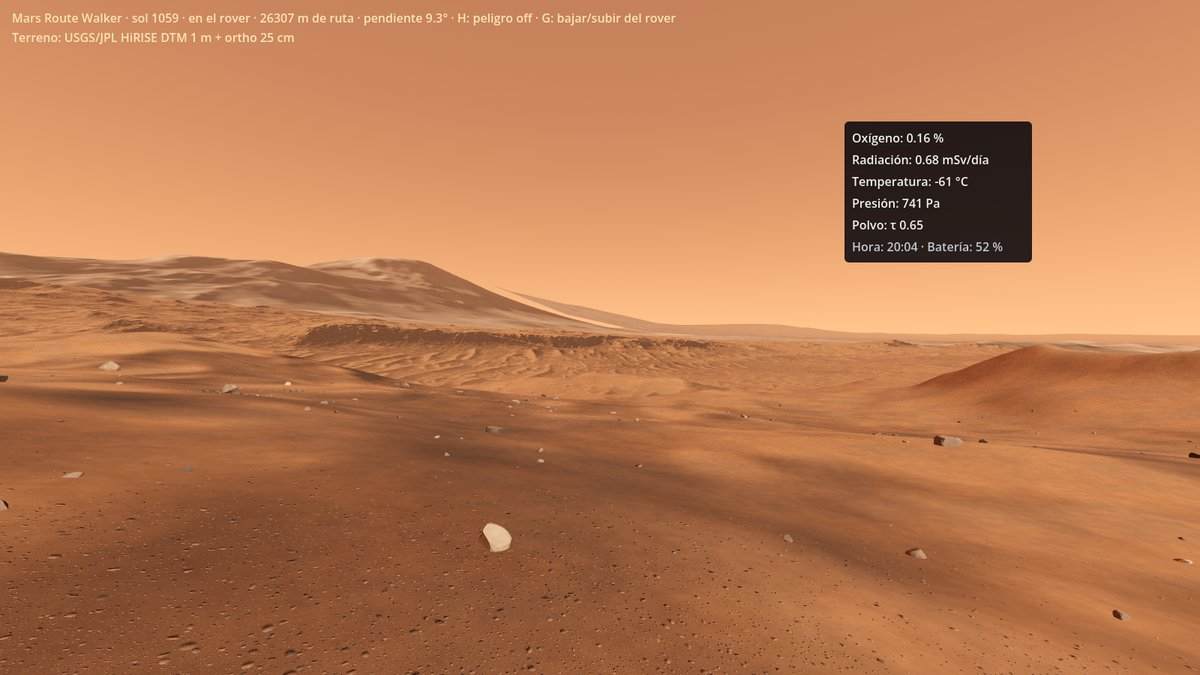
\includegraphics[width=0.49\textwidth]{figuras/escena_panel.jpg}\hfill
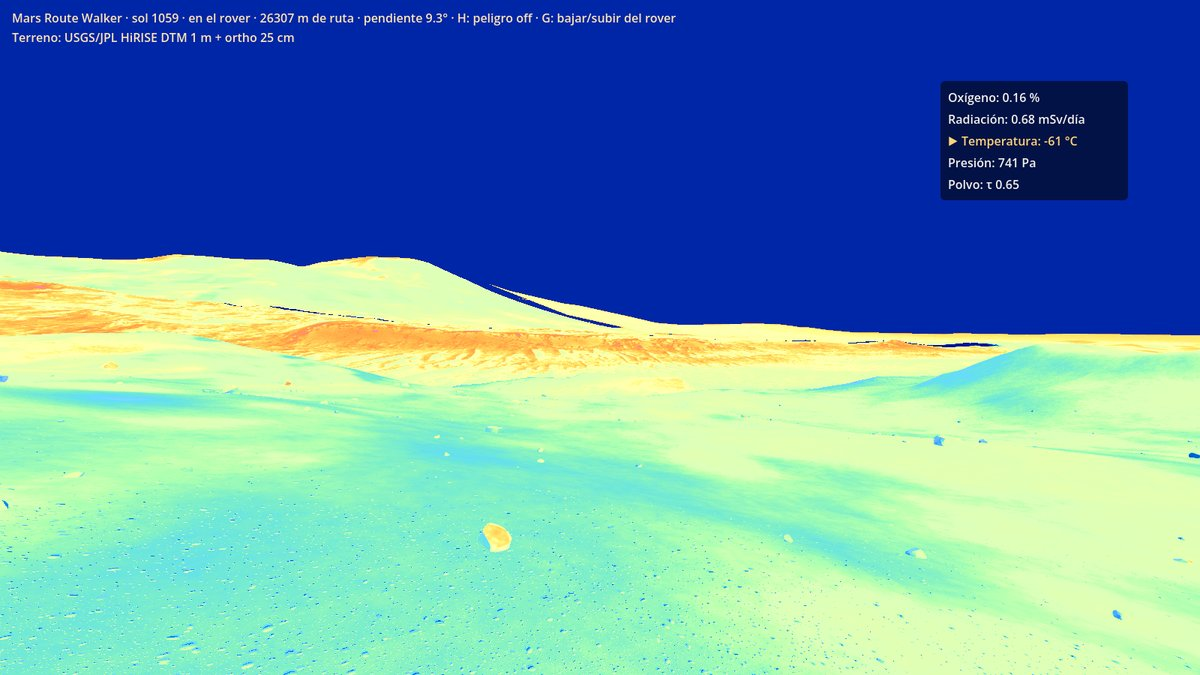
\includegraphics[width=0.49\textwidth]{figuras/vista_calor.jpg}\\[3pt]
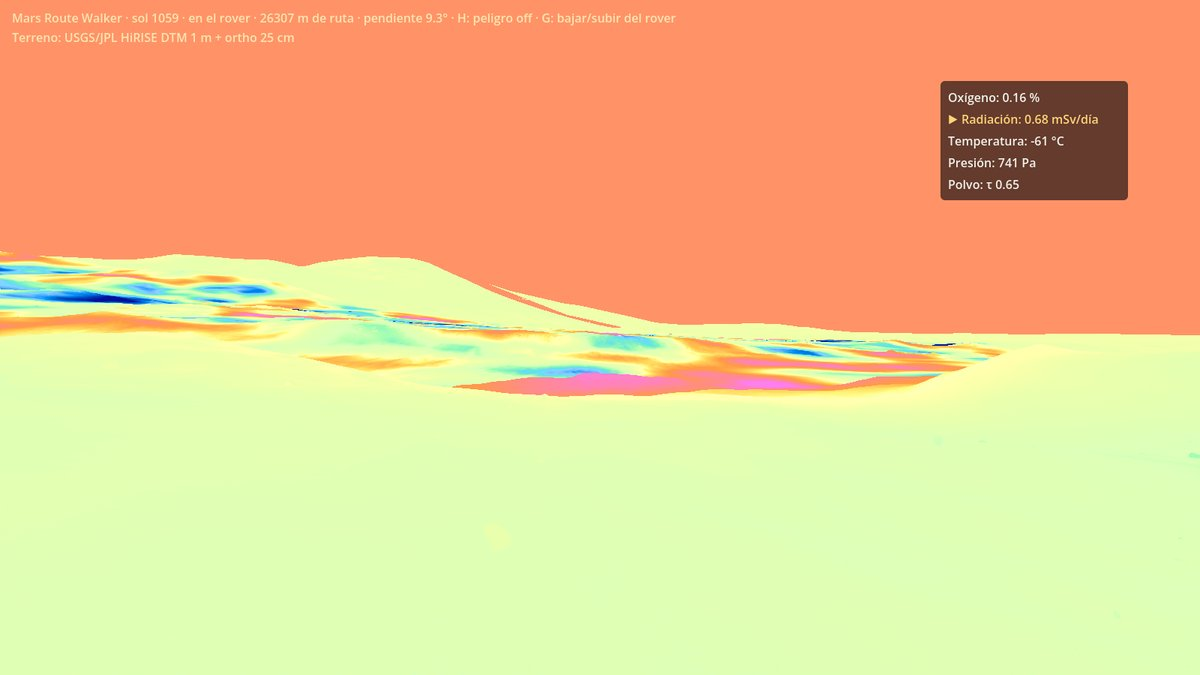
\includegraphics[width=0.49\textwidth]{figuras/vista_radiacion.jpg}\hfill
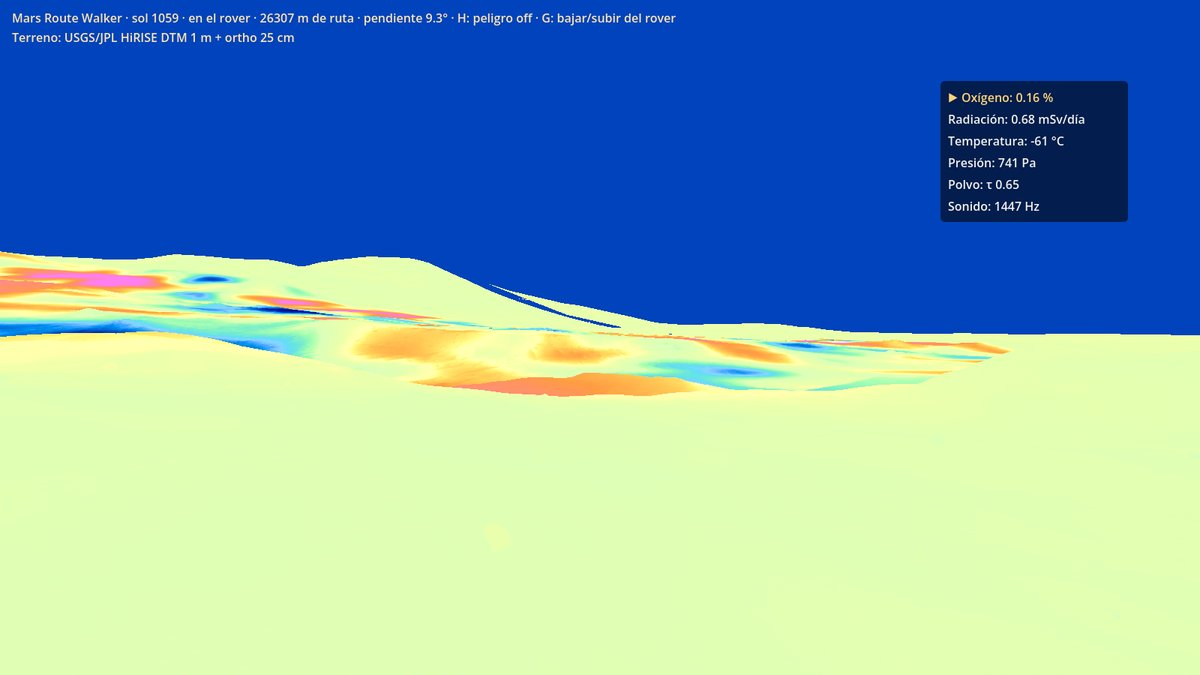
\includegraphics[width=0.49\textwidth]{figuras/vista_oxigeno.jpg}
\caption{Punto A (sol 1063). Arriba: escena con el panel de la capa (izq.) y vista de calor, tecla P (der.). Abajo: vista de radiación, tecla O (izq.) y vista de oxígeno, tecla K (der.). Paleta común: azul = menos del parámetro, magenta = más; escala automática entre los percentiles 5 y 95 del mapa.}
\label{fig:vistas}
\end{figure*}

\section{Derivadas y pendientes}\label{sec:pend}
\subsection{Diferencias centrales}
La capa de peligro del núcleo (tecla H) pinta de rojo el terreno empinado. La pendiente se obtiene del gradiente de la altura $h(x,z)$ con diferencias centrales:
\begin{equation}
\frac{\partial h}{\partial x} \approx \frac{h(x+\Delta)-h(x-\Delta)}{2\Delta} = h'(x) + \frac{\Delta^2}{6}h'''(\xi),
\end{equation}
con error de truncamiento $O(\Delta^2)$ (desarrollo de Taylor). La pendiente es
\begin{equation}
\theta = \arctan\lVert\nabla h\rVert = \arccos n_y,\qquad \mathbf n = \frac{(-h_x,\,1,\,-h_z)}{\sqrt{1+h_x^2+h_z^2}},
\end{equation}
y el color rojo crece con $\mathrm{smoothstep}(9°, 19.5°, \theta)$, alrededor del umbral de 15°. El número del HUD usa $\Delta = 1$\,m; la malla, el espaciado de su nivel de detalle.

\subsection{Respuesta en frecuencia}
Como filtro FIR, la diferencia central tiene coeficientes $[-1, 0, 1]/(2\Delta)$. Aplicada a $e^{j\omega x}$:
\begin{equation}
H(\omega) = \frac{j\sin(\omega\Delta)}{\Delta} = j\omega\,\frac{\sin(\omega\Delta)}{\omega\Delta},
\end{equation}
es decir, el derivador ideal $j\omega$ por una función $\mathrm{sinc}$: es exacto en bajas frecuencias, tiene ganancia máxima $1/\Delta$ en $\omega = \pi/(2\Delta)$ (amplifica el ruido del modelo de elevación) y se anula en Nyquist. Al aumentar $\Delta$ lejos del jugador, el filtro actúa como pasa-bajos y las pendientes cortas se promedian.

\subsection{Uso en la capa: insolación de laderas}
La capa usa el mismo gradiente (con $\Delta = 20$\,m) para la ley del coseno de Lambert. Con $\hat{\mathbf s}$ la dirección al sol, la insolación relativa de una ladera respecto al plano es $I = \max(\mathbf n\cdot\hat{\mathbf s},0)/\hat s_y - 1$, y la temperatura del lugar es
\begin{equation}
T = T_b + 4\,\mathrm{clip}(I)\,d - 5\,\mathrm{clip}\!\left(\tfrac{\Delta h_{\text{hond}}}{15}\right)(1-d) + 1.5\,n_T,
\end{equation}
con $d$ el factor de día: de día se calientan las laderas al sol y de noche el aire frío baja a las hondonadas.

\section{Visualización: integración numérica}
La neblina recorre el rayo de cada píxel y acumula la transmitancia de Beer--Lambert con $N = 24$ pasos cuadráticos $t_i = D(i/N)^2$ (cortos cerca de la cámara):
\begin{align}
\mathcal T &= \prod_{i=1}^{N} e^{-\sigma_i (t_i - t_{i-1})},\\
\sigma_i &= \kappa\,(0.015 + 5v_i^3)\,e^{-\max(y_i-h_i,0)/H_c},
\end{align}
una suma de Riemann de la integral de extinción con un perfil exponencial de altura $H_c$. Las vistas de falso color normalizan cada parámetro entre sus percentiles 5 y 95 en el mapa (ganancia automática) y compensan el \emph{tonemapping} ACES del núcleo invirtiendo su función racional $y = \frac{x(2.51x+0.03)}{x(2.43x+0.59)+0.14}$ con la fórmula cuadrática.

\section{Cálculo de rutas}
\subsection{Aproximación lineal por tramos}
La ruta de \emph{Perseverance} es una polilínea: cada segmento es la recta tangente (secante) local al camino. Su longitud es $\ell = \sum_k\lVert\mathbf p_{k+1}-\mathbf p_k\rVert$. Entre A y B la polilínea mide unos 570\,m; remuestreada cada 10\,m mide 477\,m, porque el remuestreo elimina las maniobras y zigzags de menos de 10\,m (un efecto de diezmado).

\subsection{Función de costo}
Se define el costo de un camino $\Gamma$ como la integral de línea
\begin{equation}
J = \int_\Gamma c(\mathbf x)\,ds \approx \sum_k \Delta s_k\, c(\mathbf x_k),
\end{equation}
\begin{equation}
c = 1 + w_D\,\hat D + w_O\,\hat O + w_\tau\,\hat\tau + w_\theta\left(\frac{\theta}{15°}\right)^2,
\end{equation}
con $\hat D$, $\hat O$ (falta de O$_2$) y $\hat\tau$ normalizados a $[0,1]$ con las escalas de la capa y todos los pesos iguales a 1. El término 1 hace que $J$ crezca con la distancia, y la restricción dura $\theta\le 15°$ excluye celdas.

\subsection{Búsqueda A*}
Sobre una grilla de 10\,m que cubre el tramo con 150\,m de margen ($64\times40$ celdas, 514 prohibidas por pendiente) se aplica A*~\cite{hart1968} con heurística euclidiana, admisible porque $c\ge1$. Para comparar en igualdad de condiciones, los tres caminos se evalúan con el mismo sol de referencia (1089.5) a las 08{:}29.

\begin{table}[t]
\caption{Comparación de caminos entre A (sol 1063) y B (sol 1116)}
\label{tab:rutas}
\centering\small
\begin{tabular}{@{}lrrrr@{}}
\toprule
Camino & $\ell$ (m) & $J$ & $\theta_{\max}$ & Dosis (mSv) \\ \midrule
Ruta real & 477 & 1091 & 11.0° & 0.00359 \\
Recta A$\to$B & 320 & 767 & \textbf{18.0°} & 0.00240 \\
Óptima (A*) & 335 & \textbf{752} & 11.3° & 0.00250 \\
\bottomrule
\end{tabular}
\\[2pt]\footnotesize Dosis: caminando a 1\,m/s. $p_{O_2}$ mínima $\approx 1.22$\,Pa en los tres.
\end{table}

\begin{figure}[t]
\centering
\begin{tikzpicture}
\begin{axis}[width=\columnwidth, height=5.0cm, axis equal image,
  xlabel={$x$ (m, este)}, ylabel={$-z$ (m, norte)},
  legend style={font=\scriptsize, at={(0.5,1.03)}, anchor=south, legend columns=4}, tick label style={font=\scriptsize}, label style={font=\small}]
\addplot[thick, blue] table[x=x, y expr=-\thisrow{z}, col sep=comma] {datos/ruta_real.csv};
\addplot[thick, red, dashed] table[x=x, y expr=-\thisrow{z}, col sep=comma] {datos/ruta_recta.csv};
\addplot[thick, black!70!green] table[x=x, y expr=-\thisrow{z}, col sep=comma] {datos/ruta_optima.csv};
\legend{Real, Recta, Óptima (A*)}
\end{axis}
\end{tikzpicture}
\caption{Planta de los tres caminos entre A (derecha) y B (izquierda).}
\label{fig:mapa}
\end{figure}

\begin{figure}[t]
\centering
\begin{tikzpicture}
\begin{axis}[width=\columnwidth, height=4.4cm, xlabel={distancia recorrida $s$ (m)}, ylabel={pendiente (°)},
  legend style={font=\scriptsize, at={(0.5,1.03)}, anchor=south, legend columns=4}, tick label style={font=\scriptsize}, label style={font=\small}, ymin=0]
\addplot[blue] table[x=s_m, y=pendiente_grados, col sep=comma] {datos/ruta_real.csv};
\addplot[red, dashed] table[x=s_m, y=pendiente_grados, col sep=comma] {datos/ruta_recta.csv};
\addplot[black!70!green] table[x=s_m, y=pendiente_grados, col sep=comma] {datos/ruta_optima.csv};
\addplot[gray, densely dotted, domain=0:480] {15};
\legend{Real, Recta, Óptima, límite 15°}
\end{axis}
\end{tikzpicture}
\caption{Pendiente a lo largo de cada camino. La recta supera el límite de 15°.}
\label{fig:pend}
\end{figure}

\subsection{Resultados}
La Tabla~\ref{tab:rutas} y las Figs.~\ref{fig:mapa}--\ref{fig:pend} muestran que la recta es la más corta (33\,\% menos que la ruta real) pero no es factible: cruza una pendiente de 18°. El camino óptimo la rodea con solo 15\,m más y obtiene el menor costo, 31\,\% menos que la ruta real y 2\,\% menos que la recta. Hay que leer este resultado con cuidado: la ruta real responde a objetivos científicos y a restricciones del rover que el costo no incluye, y la radiación, el oxígeno y el polvo varían de forma sintética. El método, sin embargo, queda listo para datos reales.

\section{Sistemas en variables de estado}
\subsection{Seguimiento suave del panel en VR (implementado)}
El panel no está pegado rígido a la cabeza. Su orientación $q$ sigue a la de la cabeza $q_c$ con $q_{k+1} = \mathrm{slerp}(q_k, q_{c,k}, a)$. Para ángulos pequeños, en un eje:
\begin{equation}
x_{k+1} = (1-a)\,x_k + a\,u_k,\quad y_k = x_k,\qquad a = 1 - e^{-\Delta t/\tau},
\end{equation}
es decir, $A = 1-a$, $B = a$, $C = 1$, $D = 0$ y $H(z) = a/\big(z-(1-a)\big)$. Es la discretización exacta (retenedor de orden cero) de $H(s) = 1/(\tau s+1)$: el polo $s = -1/\tau$ se mapea a $z = e^{-\Delta t/\tau}$. Con $\tau = 0.25$\,s a 90\,Hz, $z = 0.9565$, dentro del círculo unitario (estable), con establecimiento al 2\,\% en $4\tau = 1$\,s. Una zona muerta con histéresis (empieza a seguir a los 6°, se detiene bajo 1°) evita que el panel se mueva con micromovimientos de la cabeza.

\subsection{Sonido de cercanía (implementado)}
El tono es un oscilador de fase continua (NCO) con estado $\varphi_{n+1} = (\varphi_n + 2\pi f_n/f_s) \bmod 2\pi$ y salida $\sin\varphi_n$, con $f_s = 22\,050$\,Hz. La frecuencia sigue a $f = 220\cdot 2^{3\ell}$\,Hz ($\ell\in[0,1]$ es la cercanía a una zona alta) con el mismo filtro de un polo, $\tau = 80$\,ms, cuyo polo queda en $z = e^{-1/(f_s\tau)} = 0.99943$.

\subsection{Control térmico del traje (propuesto, no implementado)}
Un modelo de primer orden del traje, $C\dot T = (T_{\text{ext}} - T)/R + u$, con la temperatura exterior de la capa como perturbación y un controlador PI con estado integral $\xi$ ($\dot\xi = T_{\text{ref}} - T$, $u = K_p(T_{\text{ref}}-T) + K_i\xi$), da en lazo cerrado
\begin{equation}
\dot{\mathbf x} = \begin{bmatrix} -\frac{1}{RC}-\frac{K_p}{C} & \frac{K_i}{C}\\ -1 & 0\end{bmatrix}\mathbf x + \begin{bmatrix}\frac{K_p}{C}\\ 1\end{bmatrix}T_{\text{ref}} + \begin{bmatrix}\frac{1}{RC}\\ 0\end{bmatrix}T_{\text{ext}},
\end{equation}
con $\mathbf x = [T,\ \xi]^\top$ y polinomio característico $s^2 + \left(\frac{1}{RC}+\frac{K_p}{C}\right)s + \frac{K_i}{C}$. Las ganancias se elegirían por ubicación de polos ($\zeta$, $\omega_n$) y el lazo se discretizaría con Tustin. Queda como trabajo futuro.

\section{Conclusiones y trabajo futuro}
La capa calcula cinco parámetros con valores base medidos y leyes físicas explícitas, y los comunica con un panel mínimo y vistas de falso color. Las herramientas de ingeniería empleadas incluyen una serie de Fourier truncada, la fórmula barométrica, Beer--Lambert, diferencias centrales con análisis de error y de respuesta en frecuencia, integración numérica, búsqueda A* con una función de costo, y filtros escritos en variables de estado. Quedan como trabajo futuro: reemplazar las aproximaciones por los datos de MEDA de los sols 1063--1116 (presión, temperatura y opacidad, disponibles en el PDS), hacer avanzar la hora local con el sol de la escena, asignar botones de los controles de VR, probar la capa en el visor e implementar el lazo de control del traje.

\bibliographystyle{IEEEtran}
\bibliography{referencias}

\end{document}
